\chapter{Introduction}
\label{chap:introduction}



% Eintr�ge im Verzeichnis erscheinen lassen ohne hier eine Referenz einzuf�gen
\nocite{kopka:band1}
\nocite{raichle:bibtex_programmierung}
\nocite{MiKTeX}
\nocite{KOMA}
\nocite{TeXnicCenter}
\nocite{Marti06}
\nocite{Erbsland08}
\nocite{juergens:einfuehrung}
\nocite{juergens:fortgeschritten}

\section{Organising Documents}
\label{sec:einleitung_aufbau}
Eye tracking is used to measure where someone is looking. It is used in a wide variety of applications such as marketing research, psychology, virtual reality and sports training. 

To enable high speed eye tracking for sports the HuCE developed an eye tracking system called the Gazelle Eye Tracker that is fast, portable and built for outdoor usage. 

In figure \ref{fig:file_structure} the file structure is shown for this template.

\begin{figure}[H]
	\centering
		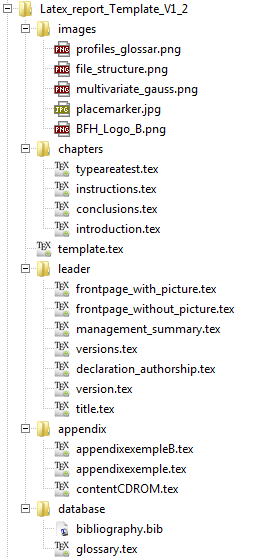
\includegraphics[scale=0.85]{images/file_structure.png}
	\caption{File structure}
	\label{fig:file_structure}
\end{figure}

\section{Contact}
\label{sec:introduction_contact}

The manufacturers of this template welcome any suggestions for improvement. Chapter \ref{sec:introduction_suggestions} shows possible suggestions for improvement\index{suggestions}.

\begin{table}[H]
	\centering
		\begin{tabular}{lll} \toprule
			\textbf{First Name Last Name} & \textbf{E-mail} & \textbf{Function} \\ \midrule
			Alfred Kaufmann & alfred.kaufmann@bfh.ch & Employer, Project Management, \\
			& & Supplements, Improvements \\ \midrule
			Fritz Dellsperger & Retired & Tips on the structure and layout \\ \midrule
			David Burri & Contracted out & First compilation of the Template \\ \bottomrule
		\end{tabular}
	\caption{Contact Persons}
	\label{tab:Contact Persons}
\end{table}


\section{Suggestions for Improvement}
\label{sec:introduction_suggestions}

\begin{itemize}
	\item Create a BFH Style Files
	\item Template for the Compilation of presentations with \LaTeX{}
\end{itemize}


